\documentclass[12pt]{article}
\usepackage[margin=1in]{geometry}
\usepackage{amsmath, amssymb, amsthm, graphicx, hyperref}
\usepackage{enumerate}
\usepackage{fancyhdr}
\usepackage{multirow, multicol}
\usepackage{tikz}
\pagestyle{fancy}
\fancyhead[RO]{Eliot Brown}
\fancyhead[LO]{MA-UY 2314: Discrete Mathematics}
\usepackage{comment}
\newif\ifshow
\showfalse

\ifshow
  \newenvironment{solution}{\textbf{Solution.}}{}
\else
  \excludecomment{solution}
\fi

\newcommand{\R}{\mathbb{R}}
\newcommand{\dydx}{\frac{dy}{dx}}
\renewcommand{\thefootnote}{\fnsymbol{footnote}}

\begin{document}

\begin{center}
\ifshow
  \textbf{\Large Homework 0 Solution}\\
\else
  \textbf{\Large Homework 0}\\
\fi
Due: Friday Feb. 7, by 11:59pm,\\via Gradescope\\
%Late HW accepted until 9PM on September 8\footnote{For each hour your homework is late, 10 points (out of 100) will be deducted from your homework score.  Please submit your homework on time!}
\end{center}

\hrule

\vspace{0.2cm}




\noindent
The purpose of this homework is twofold:
\begin{enumerate}[A.]
\item To give you an opportunity to practice submitting a homework assignment through Gradescope.  Lateness due to technical issues will not be excused.  
\item To help me gain a better idea of your goals for this course.
\item To access Gradescope via NYU Classes, click the Lessons tab followed by the Gradescope link. 
\end{enumerate}

\hrule

\vspace{0.5cm}

\noindent
Please give a brief response to each of the following question or instruction.  Parts (a)-(f) are 3 points each. Problem 2 is worth 60 points.  
\vspace{.15in}


\noindent 1.   
\begin{enumerate}
\item[(a)] Write your name and your NYU NetID (i.e., your nyu email).
 \\*  - Eliot Brown, ecb465, ecb465@nyu.edu
\item[(b)] What is your major or intended major?
 \\* - Computer Engineering 
\item[(c)] What was your most recent math course before this one and when did you take it?
 \\* - Data Analysis, last semester (Fall 2019) 
\item[(d)] Why are you taking this course?
 \\* - This course is a requirement and prerequisite 
\item[(e)] What do you hope to learn or to gain from this course?
 \\* - Different way to view mathematical concepts and thinking
\item[(f)] How did the first week of our course go for you?  (Hard or easy, fast or slow, etc.)
 \\* First week of the course was a fine pace, and was easy, but I am reading more throughout the course while it is at this slow pace, so it is good to get a head start. 
\end{enumerate}

\noindent 2.  Hand write the following below.  Include your name and signature where indicated.   
\vspace{.15in}

\noindent \textit{I}, \underline{Eliot Brown}, \textit{ understand the homework/exam structure of the course as stated in the syllabus.  In general, I understand the syllabus that has been read to me, and if and when I have a question about course structure I will read the syllabus prior to asking the professor a question.  I have been warned about the difficulties of this course.}
\vspace{.15in}

\noindent \underline{Eliot Brown}
\vspace{.15in}

\\   
\\
\[
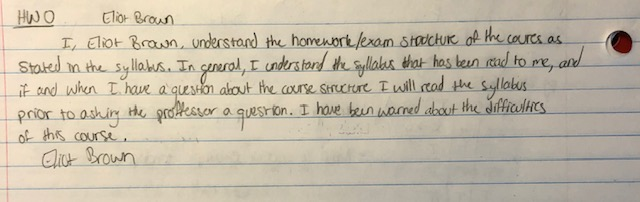
\includegraphics[width = 7in, height = 3in]{HW0Q2.jpg} %your jpg file goes between the curly brackets.  To size it, play around with the syntax between the square brackets.  
\]

\noindent \textbf{Remark:}  Problem 2 is the one problem in the semester with a strange point system attached to it.  There is a method to the madness, which I hope you will appreciate around mid March.  


\end{document}
